%% ---------------------------------------------------------------------
%% 01 - GIỚI THIỆU
%% ---------------------------------------------------------------------

\section{Giới thiệu}\label{sec:intro}

\subsection{Bối cảnh và lý do chọn đề tài}

Trong giao hàng đô thị, một robot phải đi từ kho hàng đến từng khách hàng trên
một mạng đường đã định. Khi bản đồ thành phố được dựng đủ chi tiết, mạng đường
đó không còn là đồ thị phẳng đơn thuần mà là một \textbf{bề mặt ba chiều}: địa
hình, tầng, mái và các công trình đều có bề mặt riêng. Trên bề mặt như vậy,
khoảng cách đúng giữa hai điểm không phải là đường thẳng nối trong không gian mà
là \textbf{đường đi ngắn nhất nằm trên bề mặt}. Bài toán này là một bài toán kinh
điển của hình học tính toán: tính đường đi ngắn nhất trên bề mặt đa diện
(\emph{shortest path on a polyhedral surface}).

Hai họ phương pháp thường được dùng cho bài toán lập đường có mục tiêu khác nhau.
Các phương pháp dựa trên lấy mẫu như Probabilistic Roadmap (PRM)
và RRT* tìm đường trong không gian cấu
hình, cho nghiệm tiệm cận tối ưu hoặc xác suất đầy đủ nhưng không bảo đảm độ dài
chính xác và không ràng buộc đường đi nằm trên một bề mặt cho trước. Với mô hình
thành phố đã được tam giác hóa, ràng buộc ``đi trên bề mặt'' là thông tin có sẵn
và nên được khai thác trực tiếp thay vì xấp xỉ bằng lấy mẫu.

Họ thứ hai xuất phát từ hình học tính toán. Thuật toán của Mitchell, Mount và
Papadimitriou (MMP) là mốc đầu tiên giải bài toán đường ngắn nhất trắc địa với
độ phức tạp đa thức; Chen và Han đưa độ phức tạp về $O(n^2)$ bằng kỹ thuật lan
truyền cửa sổ trên các tam giác đã trải phẳng.
Theo Phan, Hoai và Thinh, các phương pháp tiền nhiệm thường dựa trên kỹ thuật
trải phẳng (\emph{planar unfolding}): ``mở'' bề mặt đa diện ra mặt phẳng rồi mới
tính khoảng cách, nên việc xử lý các cửa sổ (\emph{window}) đòi hỏi nhiều phép
biến hình \cite{an2024funnel}. Bài báo của Phan, Hoai và Thinh (2024) đề xuất
\textbf{funnel tree}, cùng độ phức tạp $O(n^2)$ nhưng bỏ hẳn bước trải phẳng:
nhờ để đường biên trái của phễu là một \emph{straightest geodesic}, độ dài và góc
cần so sánh được tính trực tiếp trên khối ba chiều bằng định luật cos. Trên 10 bộ
dữ liệu từ 100 đến 800 đỉnh, thuật toán nhanh hơn Chen và Han 1 đến 12 lần; riêng
số nút của cây giảm từ \num{1287379} xuống \num{10401} ở bộ dữ liệu
\texttt{cube4} \cite{an2024funnel}. Hình~\ref{fig:tree-icosa} minh họa một funnel
tree: đường đi ngắn nhất từ đỉnh nguồn $s=0$ đến các đỉnh khác trên mặt
icosahedron.

\begin{figure}[!t]
  \centering
  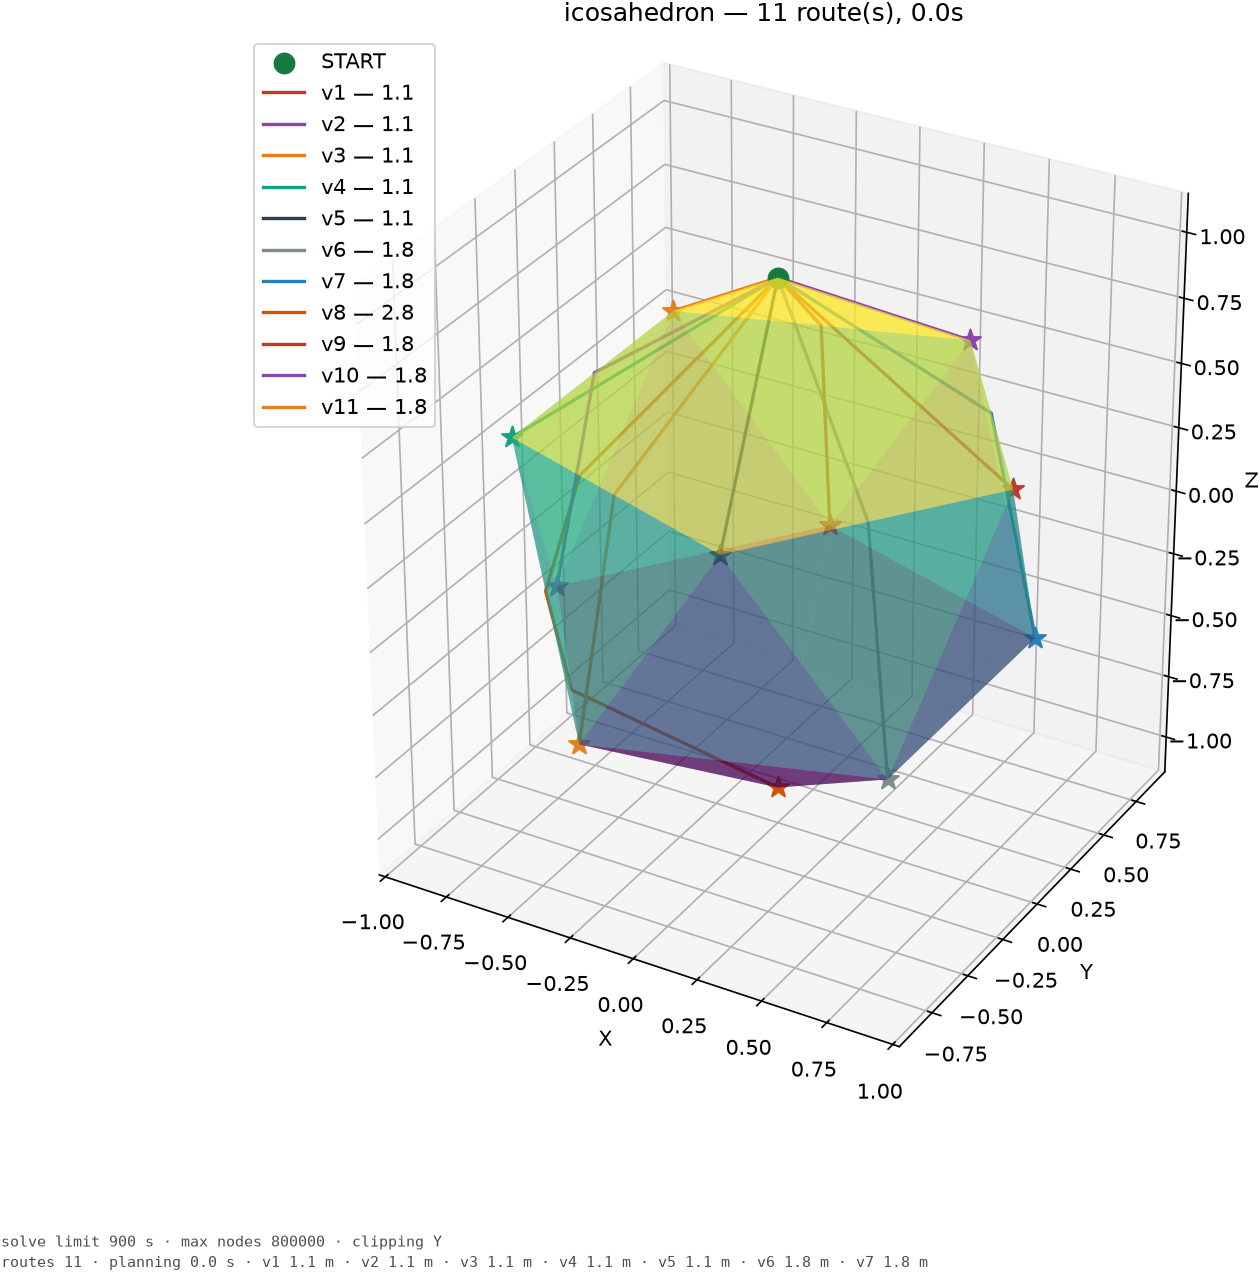
\includegraphics[width=0.9\linewidth]{Figures/crop/repo_icosahedron_routes.png}
  \caption{Các đường ngắn nhất từ đỉnh nguồn $s=0$ đến mọi đỉnh trên mặt
    icosahedron, do công cụ vẽ tuyến sinh từ route JSON của Funnel Tree. Funnel
    tree là cấu trúc sinh ra đồng thời tập đường này.}
  \label{fig:tree-icosa}
\end{figure}

Hình~\ref{fig:tree-icosa} cho thấy các tuyến tỏa từ đỉnh nguồn $s=0$ và đi qua
các mặt bên của icosahedron, không chỉ dọc theo cạnh. Một số tuyến gãy khúc tại
đỉnh có góc khuyết âm, đúng hành vi của đường trắc địa trên bề mặt lồi; đây cũng
là lý do funnel tree phải lan truyền qua mặt chứ không thể dùng đồ thị cạnh.

Đây là lựa chọn hợp lý cho bài toán giao hàng, vì funnel tree là cây ``một nguồn
đến mọi đích'', trùng trực tiếp với yêu cầu một kho hàng phục vụ nhiều khách hàng.

Về góc độ khoa học dữ liệu, bài toán là bài toán hình học -- tối ưu chứ không
phải bài toán dự đoán; phần đóng vai trò ``dữ liệu'' nằm ở khâu thực nghiệm và
đánh giá: lưới tam giác hóa (mesh) là dữ liệu vào, thời gian chạy và độ dài đường
đi là biến đo được, và việc kiểm chứng thuật toán là đối chiếu đầu ra với một
chuẩn độc lập.

\subsection{Phát biểu bài toán}

\subsubsection{Đầu vào và đầu ra}

Đầu vào của bài toán gồm:
\begin{itemize}
  \item \textbf{Bề mặt tam giác hóa} $P\subset\R^3$ gồm $n$ tam giác, cho dưới
    dạng tập đỉnh và tập mặt, mỗi cạnh kề đúng hai mặt (bề mặt kín) hoặc một mặt
    (biên của bề mặt mở);
  \item \textbf{Đỉnh nguồn} $s$;
  \item \textbf{Tập đỉnh đích} $V$ (toàn bộ đỉnh, hoặc tập con quy định trước).
\end{itemize}
Đầu ra tương ứng gồm:
\begin{itemize}
  \item Với mỗi $v\in V$: đường đi ngắn nhất toàn cục $SP(s,v)$ nằm trên $P$,
    hoặc chỉ độ dài $|SP(s,v)|$;
  \item Với bài toán đàn robot: với mỗi cặp (kho $s_i$, khách $m_j$), độ dài
    $|SP(s_i,m_j)|$ và tương ứng một lộ trình khả thi.
\end{itemize}
Độ phức tạp mục tiêu là $O(n^2)$ với $n$ là số tam giác \cite{an2024funnel}.

Bài toán này \textbf{không thuộc} nhóm phân loại, hồi quy, phân cụm, dự báo chuỗi
thời gian, gợi ý, phát hiện bất thường, xử lý ngôn ngữ tự nhiên hay thị giác máy
tính. Đây là bài toán \textbf{tìm đường đi ngắn nhất chính xác} (\emph{exact
shortest path}) trong hình học tính toán: kết quả là một đáp án đúng hay sai, có
thể đối chiếu với giá trị chính xác, không có khái niệm ``huấn luyện -- dự đoán''
hay ``độ chính xác của mô hình''.

Bản đồ thành phố được dựng thành bề mặt tam giác hóa, và trên đó các thành phần
của bài toán tổng quát được ánh xạ sang đề tài như Bảng~\ref{tab:anh-xa-de-tai}.

\begin{table}[!t]
  \caption{Ánh xạ từ bài toán chung sang đề tài.}
  \label{tab:anh-xa-de-tai}
  {\fontsize{7}{9.3}\selectfont
  \begin{tabular}{@{}>{\raggedright\arraybackslash}p{70pt}>{\raggedright\arraybackslash}p{118pt}@{}}
    \toprule
    \textbf{Thành phần bài toán} & \textbf{Tương ứng trong đề tài} \\
    \midrule
    Đỉnh nguồn $s$ & Vị trí kho hàng \\
    Đỉnh đích $v$ & Vị trí khách hàng \\
    Bề mặt tam giác hóa $P$ & Bản đồ, địa hình thành phố dưới dạng đa diện \\
    $SP(s,v)$ & Tuyến đường tối ưu từ kho đến khách \\
    $N$ nguồn đến $M$ đích & Đàn robot xuất phát từ nhiều kho phục vụ nhiều khách \\
    \bottomrule
  \end{tabular}}
\end{table}

\subsection{Mục tiêu nghiên cứu}

Mục tiêu tổng quát: lập trình một chương trình tính đường đi tối ưu cho đàn robot
xuất phát từ kho hàng đến các khách hàng trên bản đồ thành phố được dựng thành
bề mặt tam giác hóa. Các mục tiêu cụ thể, mỗi mục kèm tiêu chí kiểm chứng được,
được liệt kê trong Bảng~\ref{tab:muc-tieu}; cột trạng thái phản ánh kết quả trình
bày trong bài báo này.

\begin{table*}[!t]
  \caption{Mục tiêu nghiên cứu và tiêu chí kiểm chứng.}
  \label{tab:muc-tieu}
  {\fontsize{7}{8.6}\selectfont
  \setlength{\tabcolsep}{4pt}%
  \begin{tabular}{@{}c>{\raggedright\arraybackslash}p{150pt}>{\raggedright\arraybackslash}p{150pt}c@{}}
    \toprule
    \# & Mục tiêu cụ thể & Tiêu chí kiểm chứng & Trạng thái \\
    \midrule
    1 & Cài đặt thuật toán và Thủ tục 2 của funnel tree từ bài báo bằng Python &
      Chạy được trên toàn bộ bộ mesh kiểm thử; chỉ dùng NumPy cho mảng, không dùng
      thư viện hình học ngoài & $\checkmark$ \\
    \addlinespace
    2 & Kiểm chứng tính đúng bằng đối chiếu độc lập & (a) 5 mesh có reference
      độc lập, dung sai tương đối $10^{-4}$; (b) 4 mesh
      không có reference chỉ kiểm tra khả năng chạy và nhất quán nội tại &
      (a) $\checkmark$ \textbullet\ (b) $\triangle$ \\
    \addlinespace
    3 & Mở rộng thuật toán cho bề mặt mở & Xử lý biên nằm trong
      mã thuật toán; chạy được trên \texttt{dome} và \texttt{terrain},
      nhưng hai mesh này không có reference độc lập & $\triangle$ \\
    \addlinespace
    4 & Ghép thành bài toán nhiều nguồn -- nhiều đích cho đàn robot & Kết quả từng
      cặp (kho, khách) bằng giá trị tối ưu của cặp đó & $\times$ \\
    \addlinespace
    5 & Trực quan hóa đường đi và bản đồ thành phố & Có hình tái lập được từ mã
      nguồn đính kèm & $\checkmark$ \\
    \bottomrule
  \end{tabular}
  \vspace{2pt}

  \footnotesize\raggedright
  \emph{Chú thích cột trạng thái:} $\checkmark$~hoàn thành \textbullet{}
  $\triangle$~chưa kiểm chứng đầy đủ \textbullet{} $\times$~chưa thực hiện. Với
  mục tiêu~2, cách (a) chạy trong mã kiểm chứng; cách (b) và (c) mới ở dạng
  nguyên mẫu. Mục tiêu~3 đã kiểm chứng bằng cận trên trên hai lưới mở
  (\texttt{dome}, \texttt{terrain}) ở Mục~\ref{sec:results}.}
\end{table*}

\subsection{Cấu trúc bài báo}

Bài báo gồm các phần sau. Mục~\ref{sec:intro} giới thiệu bối cảnh, phát biểu bài
toán và mục tiêu nghiên cứu. Mục~\ref{sec:theory} trình bày kiến thức nền (bề mặt
đa diện, straightest geodesic, cấu trúc phễu), cơ sở khoa học dữ liệu, nguyên lý
thuật toán Funnel Tree cùng cơ chế cắt tỉa và các chỉ số đánh giá.
Mục~\ref{sec:data} mô tả các nguồn dữ liệu thực nghiệm, đặc tả Data Dictionary,
kết quả kiểm tra chất lượng dữ liệu, phân tích khám phá và các insight hình học.
Mục~\ref{sec:results} trình bày kết quả thực nghiệm trên các lưới đa diện, nghiên
cứu trường hợp điển hình trên địa hình vách dốc, kiểm định cơ chế cắt tỉa, phân
tích sai số số học và thảo luận. Mục~\ref{sec:gazebo} trình bày phần mô phỏng
Gazebo: dựng ba bề mặt dẫn đường từ mô hình thành phố, lập tuyến bằng Funnel Tree,
mô phỏng bám tuyến trong Gazebo và so sánh ba cấu hình lưới.
Mục~\ref{sec:concl} kết luận.
